\let\negmedspace\undefined
\let\negthickspace\undefined
\documentclass[journal,12pt,twocolumn]{IEEEtran}
%\documentclass[conference]{IEEEtran}
%\IEEEoverridecommandlockouts
% The preceding line is only needed to identify funding in the first footnote. If that is unneeded, please comment it out.
\usepackage{cite}
\usepackage{amsmath,amssymb,amsfonts,amsthm}
\usepackage{algorithmic}
\usepackage{graphicx}
\usepackage{textcomp}
\usepackage{xcolor}
\usepackage{txfonts}
\usepackage{listings}
\usepackage{enumitem}
\usepackage{mathtools}
\usepackage{gensymb}
\usepackage[breaklinks=true]{hyperref}
\usepackage{tkz-euclide} % loads  TikZ and tkz-base
\usepackage{listings}
%
%\usepackage{setspace}
%\usepackage{gensymb}
%\doublespacing
%\singlespacing

%\usepackage{graphicx}
%\usepackage{amssymb}
%\usepackage{relsize}
%\usepackage[cmex10]{amsmath}
%\usepackage{amsthm}
%\interdisplaylinepenalty=2500
%\savesymbol{iint}
%\usepackage{txfonts}
%\restoresymbol{TXF}{iint}
%\usepackage{wasysym}
%\usepackage{amsthm}
%\usepackage{iithtlc}
%\usepackage{mathrsfs}
%\usepackage{txfonts}
%\usepackage{stfloats}
%\usepackage{bm}
%\usepackage{cite}
%\usepackage{cases}
%\usepackage{subfig}
%\usepackage{xtab}
%\usepackage{longtable}
%\usepackage{multirow}
%\usepackage{algorithm}
%\usepackage{algpseudocode}
%\usepackage{enumitem}
%\usepackage{mathtools}
%\usepackage{tikz}
%\usepackage{circuitikz}
%\usepackage{verbatim}
%\usepackage{tfrupee}
%\usepackage{stmaryrd}
%\usetkzobj{all}
%    \usepackage{color}                                            %%
%    \usepackage{array}                                            %%
%    \usepackage{longtable}                                        %%
%    \usepackage{calc}                                             %%
%    \usepackage{multirow}                                         %%
%    \usepackage{hhline}                                           %%
%    \usepackage{ifthen}                                           %%
  %optionally (for landscape tables embedded in another document): %%
%    \usepackage{lscape}     
%\usepackage{multicol}
%\usepackage{chngcntr}
%\usepackage{enumerate}

%\usepackage{wasysym}
%\newcounter{MYtempeqncnt}
\DeclareMathOperator*{\Res}{Res}
%\renewcommand{\baselinestretch}{2}
\renewcommand\thesection{\arabic{section}}
\renewcommand\thesubsection{\thesection.\arabic{subsection}}
\renewcommand\thesubsubsection{\thesubsection.\arabic{subsubsection}}

\renewcommand\thesectiondis{\arabic{section}}
\renewcommand\thesubsectiondis{\thesectiondis.\arabic{subsection}}
\renewcommand\thesubsubsectiondis{\thesubsectiondis.\arabic{subsubsection}}

% correct bad hyphenation here
\hyphenation{op-tical net-works semi-conduc-tor}
\def\inputGnumericTable{}                                 %%

\lstset{
%language=C,
frame=single, 
breaklines=true,
columns=fullflexible
}
%\lstset{
%language=tex,
%frame=single, 
%breaklines=true
%}

%\documentclass{article}
\usepackage{geometry}
\geometry{a4paper, margin=2cm}
\usepackage{listings}

\begin{document}

\title{Report for My Music Player code}
\author{Muppalla Bhavesh Chowdary\\
CS22Btech11041
}
\date{\today}
\maketitle

\section{Introduction}
This document provides an explanation of a simple music player implemented using the Python programming language and the Tkinter and Pygame libraries.

\section{Code Explanation}

\subsection{Importing Libraries}
The code begins by importing the necessary libraries: \texttt{Tkinter} and \texttt{mixer} from \texttt{pygame}, \texttt{prog} (presumably a user-defined module), \texttt{random}, and \texttt{time}.

\subsection{Initializing the Mixer}
The \texttt{mixer.init()} function is called to initialize the audio mixer from the \texttt{pygame} library.

\subsection{Print Statement}
The line \texttt{print(prog.finalarr)} outputs the value of the \texttt{finalarr} variable from the \texttt{prog} module.

\subsection{Play Function}
The \texttt{play} function takes a \texttt{song} parameter, which is used to construct the file path of the corresponding MP3 file. The \texttt{mixer.music.load()} function loads the MP3 file, and \texttt{mixer.music.play()} starts playing the music.

\subsection{Play All Function}
The \texttt{playall} function plays all the songs in the \texttt{finalarr} list of the \texttt{prog} module. It calls the \texttt{play} function for each song, incrementing the \texttt{songindex} variable in the \texttt{prog} module after each song is played.

\subsection{Pause and Resume Functions}
The \texttt{pausesong} function pauses the currently playing music using \texttt{mixer.music.pause()}, and the \texttt{resumesong} function resumes the paused music using \texttt{mixer.music.unpause()}.

\subsection{Next Song Function}
The \texttt{nextsong} function stops the currently playing music with \texttt{mixer.music.stop()} and proceeds to play the next song in the \texttt{finalarr} list, similar to the \texttt{playall} function.

\subsection{Randomizer algorithm}

\subsubsection{Importing Libraries}
The code snippet begins by importing the necessary libraries: \texttt{numpy} as \texttt{num}, \texttt{playsound}, and \texttt{math}.

\subsubsection{Array Initialization}
Two arrays are initialized with 20 elements each:
\begin{itemize}
  \item \texttt{arr}: An array filled with zeros.
  \item \texttt{finalarr}: An array filled with zeros.
\end{itemize}

\subsubsection{Variable Initialization}
Two variables are initialized:
\begin{itemize}
  \item \texttt{index}: A counter variable starting from 0.
  \item \texttt{songindex}: Another counter variable starting from 0.
\end{itemize}

\subsubsection{Randomization Loop}
The code enters a \texttt{while} loop that continues until \texttt{index} reaches 20. Within each iteration of the loop, the following steps are performed:
\begin{enumerate}
  \item Generate a random number between 0 and 20 using \texttt{num.random.uniform(0, 20)}.
  \item Floor the random number to the nearest integer using \texttt{math.floor(dummy)}.
  \item Check if the element at the randomly generated index (\texttt{dummy}) in the \texttt{arr} array is 0.
  \item If the condition is true, assign the value of \texttt{dummy} to the corresponding index in the \texttt{finalarr} array.
  \item Set the element at the \texttt{dummy} index in the \texttt{arr} array to 1.
  \item Increment the \texttt{index} variable by 1.
\end{enumerate}

\subsection{GUI Initialization}
The code creates a Tkinter window using \texttt{Tk()}, sets its geometry and title, and makes it non-resizable.

\subsection{Button Widgets}
Five buttons are created using the \texttt{Button} class, with labels "Play", "Pause", "Resume", "Next", and "Randomize". Each button is associated with a specific function (\texttt{playall}, \texttt{pausesong}, \texttt{resumesong}, \texttt{nextsong}, and \texttt{randomizer}) using the \texttt{command} parameter.

\subsection{Song Information}
The information of the currently playing song is displayed below the "Next" button.

\subsection{Window Update and Main Loop}
The \texttt{root.update()} function updates the window, and \texttt{root.mainloop()} starts the Tkinter event loop, which keeps the window visible and processes user interactions until the program is terminated.

\subsection{output}
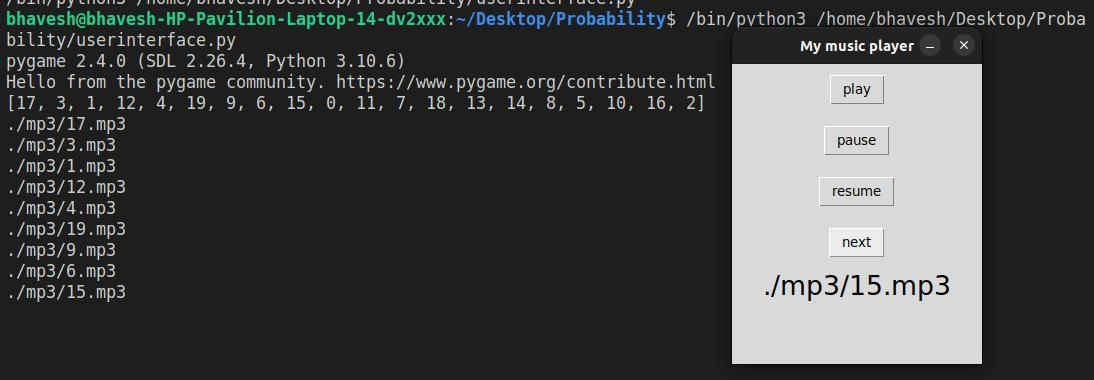
\includegraphics[scale=0.25]{./output.jpg}

\end{document}
